\chapter{Work to Date\label{chap:work2date}}
  During the months since the inception of this PhD, a wide domain crossing multiple fields has been explored. This exploration of fields utilising complex system simulations has culminated in guiding the research towards a central topic of benefit to a wide range of fields: spatial data-structure's capable of handling dynamic data. This early research exposed the bottlenecks apparent in many complex simulations that rely on the interaction of mobile spatial agents, and a dearth of research into methods for the efficient handling of dynamic spatial data.
  
  The below sections provide greater detail on how the areas covered lead to the central topic of this thesis.
  
 \section{Pedestrians}
    Pedestrian and crowd modelling, as described in Section \ref{sub:ped-modelling}, are a complex simulation whereby spatial agents (pedestrians) are constrained to a 2.5 dimensional environment and must avoid other pedestrians and the environment whilst traversing towards a goal.
    
    The initial interaction with pedestrian modelling was concerned with the effectiveness of different techniques used for global navigation, comparing their memory-overhead, precision and performance trade-offs. In benchmarking these algorithms however, it became apparent that it was the local navigation (also known as collision avoidance) which would often occupy the majority of execution time (upwards of 50\%).
    
    These local navigation models are concerned with allowing pedestrian agents to avoid collisions with other dynamic agents, most often other pedestrians although in more complex models these may include vehicles and similar.
    
    The reason that they require significantly more execution than global navigation, is that global navigation models generally lookup direction data related to their current location and target destination (whether this be via a discrete map or a grid system). Local navigation however, iteratively calculates an avoidance force based on other nearby dynamic agents. This alone requires many scattered memory reads, and becomes worse as the density of dynamic agents increases (as each agent then surveys a greater number of neighbours).
    
    A summary of this global navigation comparison was optimistically submitted to AAMAS, however two of the three reviewers felt the paper lacked substantial novelty. The full paper is available in appendix A.%\pageref{appendix:a}\&\ref{appendix:a}\&\ref{appendix:b}.
    
    \subsection*{Oliva \& Pelechano}
    Additionally techniques for generating (global) navigation graphs were investigated. It was found that the work of Oliva \& Pelechano\cite{OP11,OP12,OP13}, appeared to far surpass the limitations of the earlier work by by Pettr\'{e} et al\cite{PLT05} displaying near optimal navigation graphs generated for arbitrary 3d models. 
    
    The algorithm described in Oliva \& Pelechano 2013\cite{OP13}, consists of many steps utilising the graphics pipeline. The entire algorithm converts the walkable areas of a 3d model into a mesh of convex polygons which can be used as a navigation graph.
    
    \subsubsection*{Algorithm}
    
      A simple model with multiple walkable layers is designed and exported in wavefront (.obj) format so that it can be imported into an OpenGL scene [Fig. \ref{fig:step-1}].
      
      The model is scaled and translated so that it fits within 50 units of the origin in each direction. This area is then decomposed into an axis-aligned 3-dimensional grid of 100x100x100 voxels, these are initialised to an empty state. Each voxel plane (1x100x100 voxels) along each of the three axis, is then rendered to detect whether the relevant voxels contain any fragments. This is achieved by rendering each voxel via an orthographic projection without lighting to a 100x100 texture. The near and far clipping planes are configured such that only fragments within the desired plane of voxels are rendered. The original paper suggested this should be completed twice for each voxel plane, each direction along it's axis, however by rendering both front and back polygons this only need be completed once per voxel plane.
      
      Each pixel from each rendered texture is read, if a colour other than the clear colour is found, the relevant voxel is set to an active state [Fig. \ref{fig:step-2}].
      
      The above algorithm is then updated so that custom shaders are used, allowing the angle of each fragment to be detected. By passing the interpolated world coordinates of each vertex to the fragment shader, it is possible to calculate the face normal of each fragment. The angle between the face normal and the up vector is then compared. If this angle is less than 30 degrees the fragment is painted green to denote that it is walkable, otherwise it is painted red (this denotes the voxel is occupied but not walkable, as unoccupied voxels contain no fragments to be rendered) [Algorithm \ref{fig:slice-shader}].

\begin{algorithm}
\begin{lstlisting}[language=GLSL]
#version 330 core
in vec3 u_normal;
out vec3 color;
void main(){
	vec3 faceNorm = normalize(cross(dFdx(u_normal), dFdy(u_normal)));
	vec3 upNorm = vec3(0.0,1.0,0.0);
	float cos_angle = dot(faceNorm,upNorm)/(length(faceNorm)*length(upNorm));
	color = (cos_angle>0.86)?vec3(1,0,0):vec3(0,1,0);
}
\end{lstlisting}
\protect\caption{\label{fig:slice-shader}Fragment shader for detecting walkable fragments.}
\end{algorithm}

      Subsequently the processing of rendered textures must be updated so that voxels are marked as walkable or not walkable instead of active. After the map of walkable voxels has been completed, it is processed to mark occluded walkable voxels as not walkable. A walkable voxel is found to be unwalkable if another active voxel is within the 10 voxels directly above. Within a real-world model, this value would be adjusted to the scale of a human height [Fig. \ref{fig:step-3}].

      The walkable voxels are then flood filled from a known walkable point. Any voxels which are not filled are then marked as inaccessible [Fig. \ref{fig:step-4}].
      
      Next the distinct walkable layers are then extracted from the voxel map. This is achieved by utilising a modified flood fill, whereby a voxel is only filled if it is the first voxel in it's column to be filled with the value for the current layer. Once the modified flood fill completes, if the voxel map still contains a walkable voxel not assigned a layer, the current layer counter increases and the flood fill restarts at this layer. The voxel map now can now be overlaid on the model showing the detected walkable areas [Fig. \ref{fig:step-5}].

      All voxels which have not been assigned a walkable layer are then culled by marking them as empty. The walkable voxels are then iterated again, marking neighbouring empty voxels as part of their walkable layer [Fig. \ref{fig:step-6}]. Voxels are marked into a temporary map, which is then merged to prevent accidental chaining of expansion. This stage ensures that all possible walkable fragments are accounted for, that may have been missed at earlier stages.
      
      Now the voxel map is stored in texture memory so that it can be accessed by the shaders. The original model is now rendered using another pair of custom shaders. This fragment shader calculates the world coordinate of the fragment. This is then mapped into the voxel map stored in texture memory, so the state of the relevant voxel can be read. If this voxel is identified as being a member of a walkable layer the fragment is painted the relevant colour, else the fragment is discarded (so that it isn't rendered) [Fig. \ref{fig:step-8}].
    \begin{figure}
\protect\caption{Visible stages of the walkable surface extraction algorithm as reproduced from Oliva \& Pelechano 2013 \cite{OP13}}
%\begin{centering}
%\ContinuedFloat
%\par\end{centering}

\begin{centering}
\subfloat[\label{fig:step-1}Initial model.]{

\centering{}\includegraphics[width=0.5\columnwidth]{\string"../resources/navgraph/crop/0-crop\string".png}}
\par\end{centering}

\begin{centering}
\subfloat[\label{fig:step-2}Voxel decomposition.]{\begin{centering}
\includegraphics[width=0.5\columnwidth]{\string"../resources/navgraph/crop/1a-crop\string".png}\includegraphics[width=0.5\columnwidth]{\string"../resources/navgraph/crop/1b-crop\string".png}
\par\end{centering}

}
\par\end{centering}

\centering{}\subfloat[\label{fig:step-3}Walkable surface detection.]{\begin{centering}
\includegraphics[width=0.5\columnwidth]{\string"../resources/navgraph/crop/2a-crop\string".png}\includegraphics[width=0.5\columnwidth]{\string"../resources/navgraph/crop/2b-crop\string".png}
\par\end{centering}

}
\end{figure}


\begin{figure}
\ContinuedFloat
%\protect\caption{(continued) Visible stages of the walkable surface extraction algorithm as reproduced from Oliva \& Pelechano 2013 \cite{OP13}}
\begin{centering}
\subfloat[\label{fig:step-4}Accessible walkable surface detection.]{\begin{centering}
\includegraphics[width=0.5\columnwidth]{\string"../resources/navgraph/crop/3a-crop\string".png}\includegraphics[width=0.5\columnwidth]{\string"../resources/navgraph/crop/3b-crop\string".png}
\par\end{centering}

}
\par\end{centering}

\begin{centering}
\subfloat[\label{fig:step-5}Floor division.]{\begin{centering}
\includegraphics[width=0.5\columnwidth]{\string"../resources/navgraph/crop/4a-crop\string".png}\includegraphics[width=0.5\columnwidth]{\string"../resources/navgraph/crop/4b-crop\string".png}
\par\end{centering}

}
\par\end{centering}

\centering{}\subfloat[\label{fig:step-6}Contour expansion]{\begin{centering}
\includegraphics[width=0.5\columnwidth]{\string"../resources/navgraph/crop/5a-crop\string".png}\includegraphics[width=0.5\columnwidth]{\string"../resources/navgraph/crop/5b-crop\string".png}
\par\end{centering}

}
\end{figure}


\begin{figure}
\ContinuedFloat
%\protect\caption{(continued) Visible stages of the walkable surface extraction algorithm as reproduced from Oliva \& Pelechano 2013 \cite{OP13}}

% \begin{centering}
% \subfloat[\label{fig:step-7}]{\begin{centering}
% \includegraphics{\string"../resources/navgraph/crop/9-crop\string".png}
% \par\end{centering}

% }
% \par\end{centering}

\centering{}\subfloat[\label{fig:step-8}Walkable polygons, partitioned into floors.]{\begin{centering}
\includegraphics{\string"../resources/navgraph/crop/10-crop\string".png}
\par\end{centering}
}
\end{figure}
% \begin{figure}[\label{fig:oliva-pelechano}]
% \begin{centering}
% \protect
% \caption{Three stages of the walkable floor extraction algorithm:\\(a) The input model showing two walkable surfaces with a ramp connecting them.\\(b) The voxels containing polygons rendered over the model. Pink and green denote two walkable surfaces, the walkable surfaces are separated such that no two voxels in a walkable surface are in the same column. Yellow denotes a walkable surface that cannot be reached and blue denotes polygons at too steep an angle or lacking adequate space above to be walked on.\\(c) A rendering containing only the walkable surfaces of the input model.}
% \ContinuedFloat
% \par\end{centering}
% \begin{centering}
% \subfloat[\label{fig:step-1}]{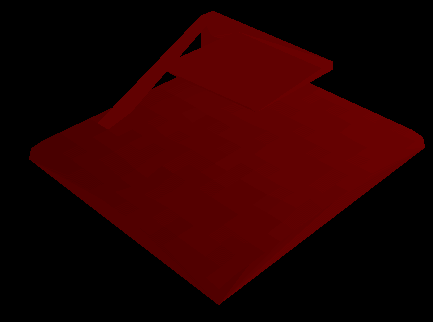
\includegraphics[width=0.5\columnwidth]{../resources/navgraph/crop/0-crop.png}}\subfloat[\label{fig:step-2}]{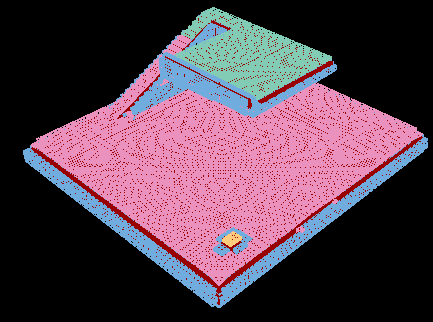
\includegraphics[width=0.5\columnwidth]{../resources/navgraph/crop/4a-crop.png}}
% \par\end{centering}
% \centering{}\subfloat[\label{fig:step-3}]{\begin{centering}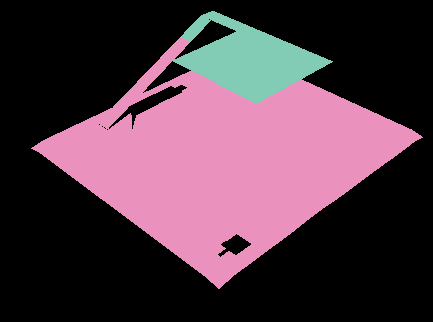
\includegraphics[width=0.5\columnwidth]{../resources/navgraph/crop/10-crop.png}
% \par\end{centering}}
% \end{figure}

  \section{Traffic}
    In contrast to pedestrian modelling, traffic modelling as described in section \ref{sub:traffic-modelling} is primarily concerned with the behaviour of spatial agents constrained to a graph (e.g. the road network). This is further complicated by the requirement that modelling accounts for complex road features, such as individual lane details which drastically increase the complexity of a real-world model in comparison to toy models before even considering vehicular agents.
    
    The initial work with traffic models, was concerned with the validity of microscopic traffic models at a large scales. A comprehensive review of traffic modelling techniques was carried out. However it became clear that without direct access to an existing implementation and model, creating an appropriately complicated scenario would divert significant research time. 
    
    It's logical that implementations would store vehicles in queues representative of a lane or road, rather than directly utilising a spatial data-structure, ensuring vehicles are constrained to the road network. This can be seen within the open-source SUMO application\cite{SUMO}, however most traffic modelling software is proprietary such that this cannot be confirmed further. In this logical format however, the fact vehicles must be responsive to other vehicles outside their own lane (and even road at intersections), can significantly increase the number of dynamic agents that must be surveyed before an agent makes a decision. As these agents would need to consider vehicles from 2 or more neighbouring queues where direct access may not be feasible.
    
    Therefore it is possible that optimisations to spatial data-structures, could make the usage of spatial data-structures for traffic modelling more attractive. There are however not currently any benchmarks to support this hypothesis by outlining the current differences between the two techniques.
    
    \section{Summary}
      The two above fields both lend credence to the benefits for efficient spatial data handling techniques. Furthermore \gls{sph} represents a field which provides a very abstract and unconstrained environment in which these same spatial data handling techniques would be beneficial. Although less attention has currently been given to \gls{sph} in comparison to pedestrian and traffic modelling within this thesis, it has been shown that \gls{sph} relies on the same spatial partitioning techniques as can be found throughout other spatial agent models.

    